The aim of the experiments was to explore the impact of
different implementations of risk group dynamics on model outputs
in a generalized epidemic model.
We compare the projected incidence and prevalence across
four model variants and range of turnover magnitudes,
as well as the estimated TPAF of the high risk group, with and without turnover.
% ==================================================================================================
\subsection{Model Variants}\label{ss:res-variants}
Figure~\ref{fig:compare-hetero-prevalence} shows the prevalence predicted by the model
with and without population heterogeneity (V1~vs~V3).
As previously noted in numerous discussions of core group theory~\citep{Yorke1978,Stigum1994},
epidemic characteristics are dramatically impacted by the presence of
heterogeneity in risk within a population.
In this case, failure to model heterogeneity in risk (V3) results in
a basic reproduction number $R_0 < 1$, and no epidemic,
while the model with heterogeneity (V1) predicts an endemic prevalence of over 12\%.
\par
Figure~\ref{fig:compare-growth-prevalence} shows the prevalence predicted by the model
with and without population growth (V1~vs~V4).
Since all model entrants are assumed to be susceptible,
simulated population growth reduces the proportion of possible contacts who are infected,
and so the relative epidemic spread is reduced,
both in terms of incidence and equilibrium prevalence.
\par
\begin{figure}
  \centering
  \begin{subfigure}{0.49\linewidth}
    \centering
    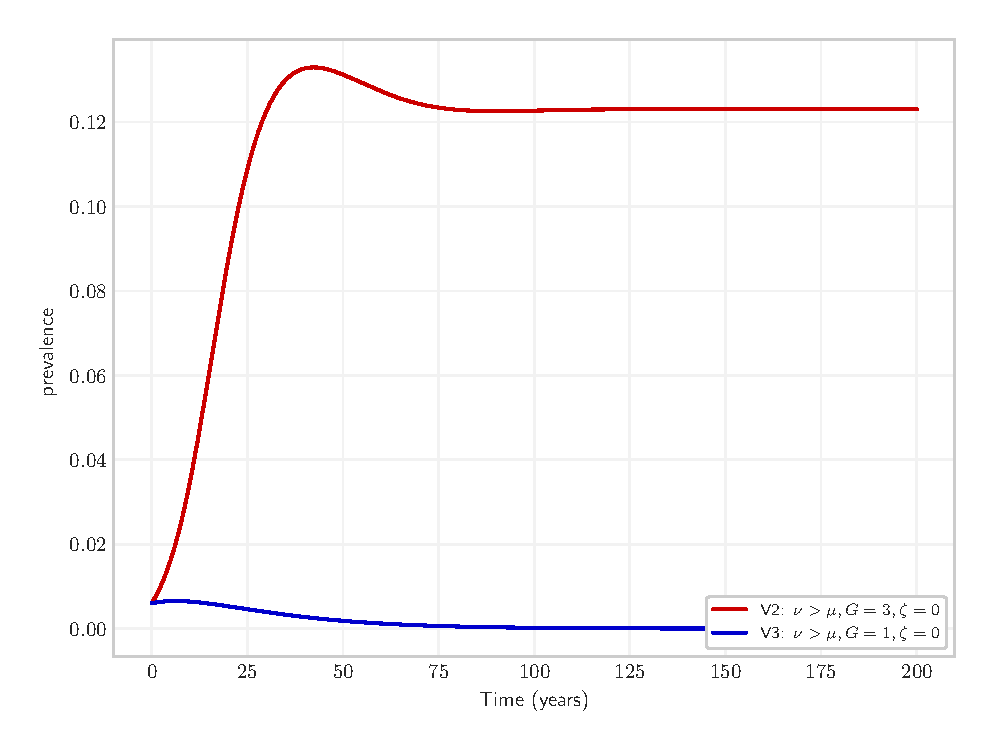
\includegraphics[width=\linewidth]{compare-hetero-prevalence}
    \caption{Risk heterogeneity (V1~vs~V3)}
    \label{fig:compare-hetero-prevalence}
  \end{subfigure}
  \begin{subfigure}{0.49\linewidth}
    \centering
    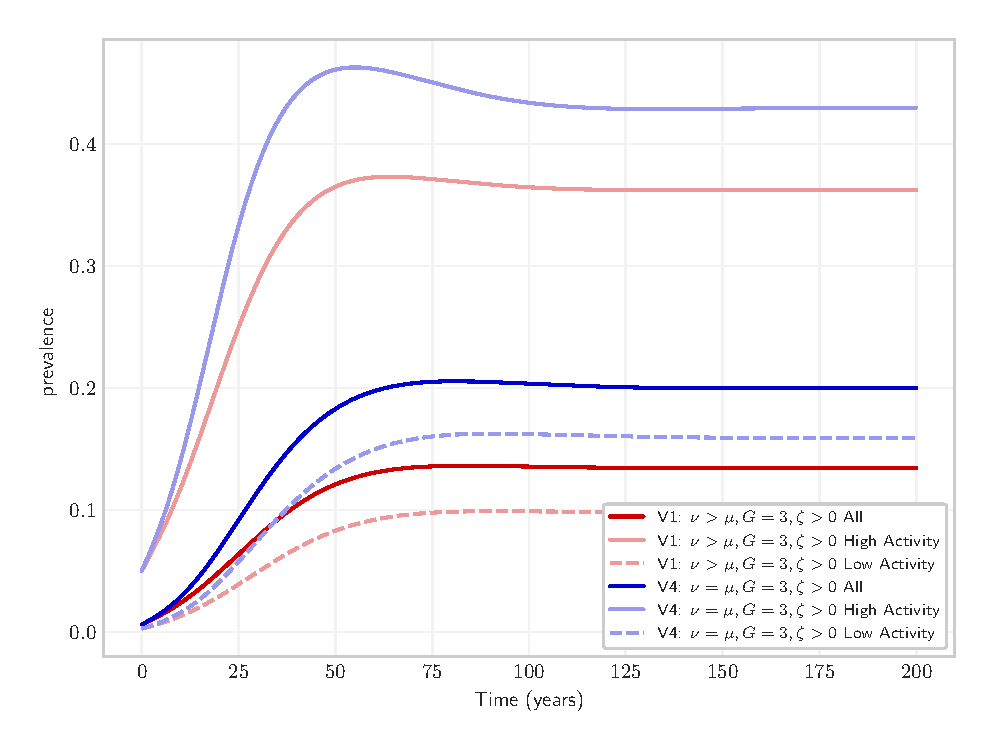
\includegraphics[width=\linewidth]{compare-growth-prevalence}
    \caption{Population growth (V1~vs~V4)}
    \label{fig:compare-growth-prevalence}
  \end{subfigure}
  \caption{Comparison of model projections with and without structural model features}
\end{figure}
\par
% TODO: add citations?
Next, we consider the impact of risk group turnover.
From Figure~\ref{fig:compare-turnover-prevalence-all},
we can see that the impact on overall equilibrium prevalence is not obvious,
and that the effects on high versus low risk groups are opposite for this system
(Figures~\ref{fig:compare-turnover-prevalence-high}~and~\ref{fig:compare-turnover-prevalence-low}).
We can observe, however, that initial epidemic spread is slowed for all groups,
as the concentration of the epidemic in a core group is eroded by 
decreasing duration of exposure in the high risk group.
In general, we might summarize this effect as a ``risk-homogenizing'' effect,
or the opposite of increased risk heterogeneity.%
\footnote{In fact, it can be shown that for sufficiently high rates of risk-group turnover,
  model outputs converge on those outputs predicted by
  a model without stratification of risk groups at all.
  This result is shown in Figure~\ref{fig:prev-converge}.}
In order to characterize additional trends, we look to the next section,
where a wider range of epidemic contexts are explored,
in terms of durations in each risk group and durations of disease infectiousness.
\par
\begin{figure}
  \centering
  \begin{subfigure}{0.31\linewidth}
    \centering
    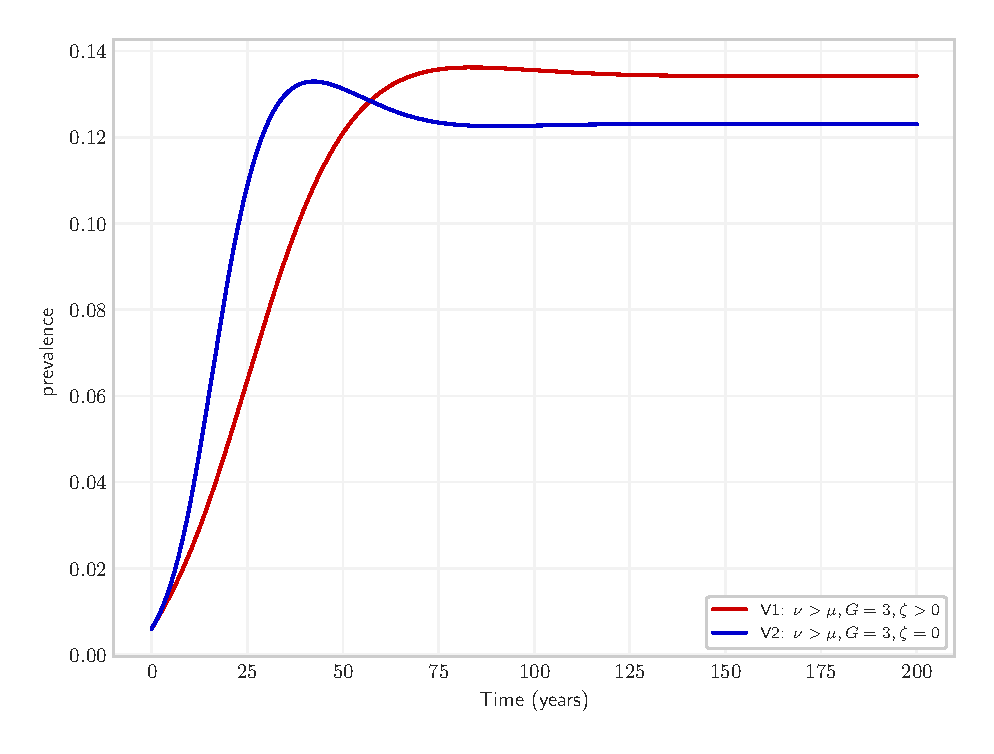
\includegraphics[width=\linewidth]{compare-turnover-prevalence-all}
    \caption{Overall}
    \label{fig:compare-turnover-prevalence-all}
  \end{subfigure}
  \begin{subfigure}{0.31\linewidth}
    \centering
    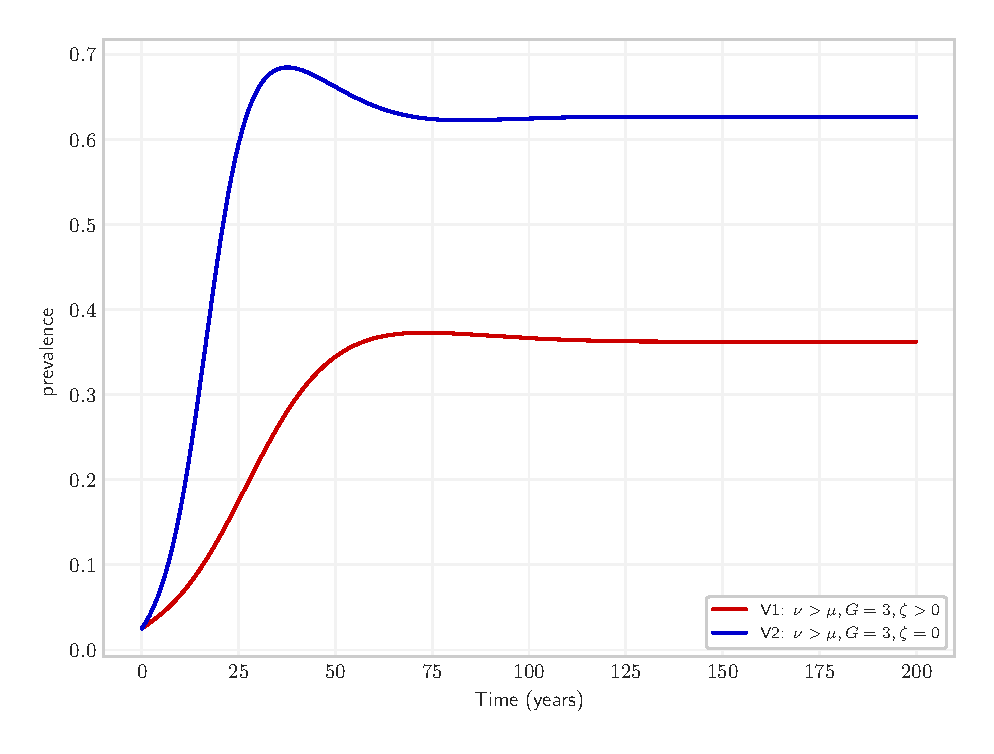
\includegraphics[width=\linewidth]{compare-turnover-prevalence-high}
    \caption{High risk}
    \label{fig:compare-turnover-prevalence-high}
  \end{subfigure}
  \begin{subfigure}{0.31\linewidth}
    \centering
    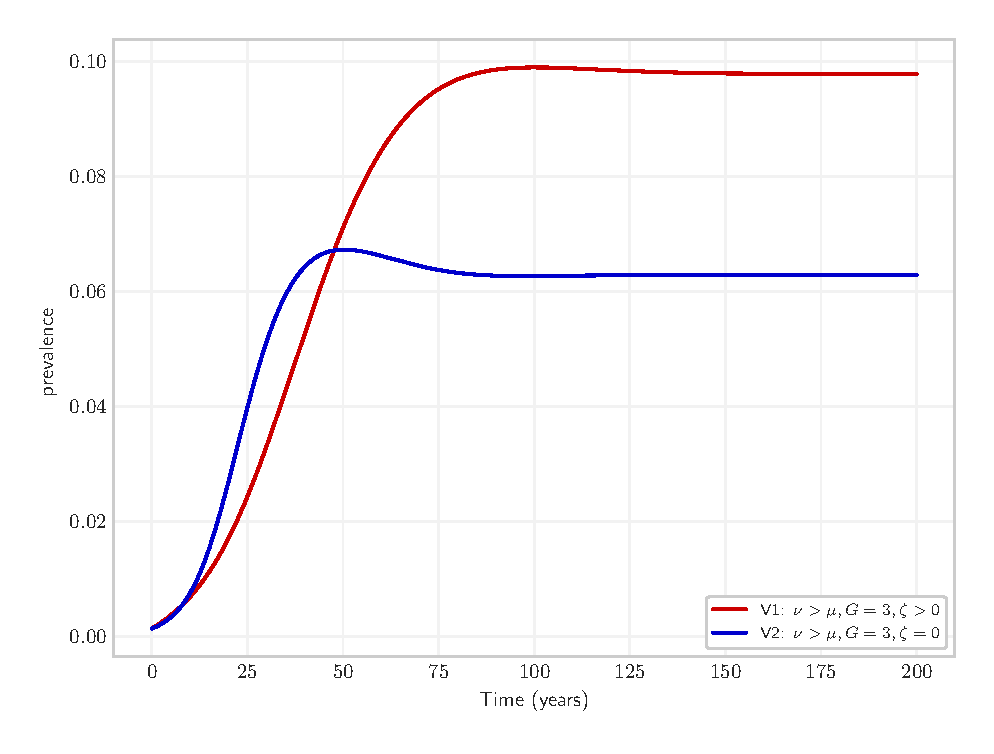
\includegraphics[width=\linewidth]{compare-turnover-prevalence-low}
    \caption{Low risk}
    \label{fig:compare-turnover-prevalence-low}
  \end{subfigure}
  \caption{Comparison of projected prevalence with and without risk group turnover (V1~vs~V2)}
  \label{fig:compare-turnover-prevalence}
\end{figure}
% ==================================================================================================
\subsection{Impact of Turnover}\label{ss:res-turnover}
Figure~\ref{fig:surface} shows the equilibrium prevalence and incidence
across a wide range of turnover rates and durations of infectiousness,
stratified by high and low risk groups, as well as overall.
We note that increasing the duration of infectiousness
increases prevalence and incidence across all groups, regardless of turnover.
However, the impact of increasing rates of turnover
can depend on the duration of infectiousness,
making it difficult to anticipate the effect of including or omitting turnover in a model.
% TODO: introduce 1D plot of simpler results first? (d_I = 10)
\par
One exception is that prevalence among the high risk group
always decreases with turnover
(Figure~\ref{fig:surface-prevalence-high}),
since the duration of exposure in this group decreases.
Turnover also increases movement of infected individuals
into low risk groups from the high risk group,
and movement of mainly susceptible individuals from low to high risk groups.
When prevalence in the high risk group is high,
the additional susceptible individuals are quickly infected,
increasing incidence in the high risk group
(Figure~\ref{fig:surface-incidence-high}, top left).
Movement of infected individuals from high to low risk groups also contributes
a considerable proportion of prevalent infections in the low risk group under these conditions
(Figure~\ref{fig:surface-prevalence-low}, top left, and Figure~\ref{fig:new-inf-L}).
However, if prevalence in the high risk group is sufficiently low,
due to short duration of infectiousness or very high turnover,
then the replacement of infected individuals with mainly susceptible individuals through turnover
decreases, rather than increases, incidence in the group
(Figure~\ref{fig:surface-incidence-high}, bottom left).%
\footnote{For simple SI* models, incidence is maximized when $\mathcal{S} = \mathcal{I}$.}
As a result, the ability of the ``core-group'' to maintain the epidemic declines,
and both incidence and prevalence decrease across all groups as turnover increases
(Figure~\ref{fig:surface}, all panels, bottom left).
Thus, for short durations of infectiousness, or for very high turnover,
no epidemic is observed, and we infer that $R_0 < 1$.
% % JK: this belongs in discussion?
% These trends echo previous observations \citep{Zhang2012,Henry2015}
% but highlight the dependence of the threshold effect on the duration of infectiousness.
% Furthermore, this implies that the rate of treatment required to achieve epidemic control
% is affected by turnover.
% Namely, since turnover acts to erode the core-group effect,
% the rate of treatment required to achieve epidemic control will be
% lower with turnover than without.
% Models which fail to capture turnover dynamics might therefore be liable to
% overestimate the treatment rate required to achieve epidemic control.
% % repetitive wording here ...
\begin{figure}
  \centering
  \begin{subfigure}{0.31\linewidth}
    \centering
    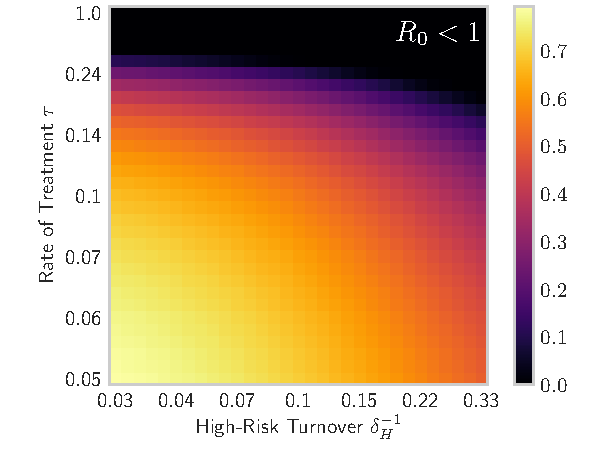
\includegraphics[width=\linewidth]{surface-prevalence-high}
    \caption{High risk prevalence}
    \label{fig:surface-prevalence-high}
  \end{subfigure}
  \begin{subfigure}{0.31\linewidth}
    \centering
    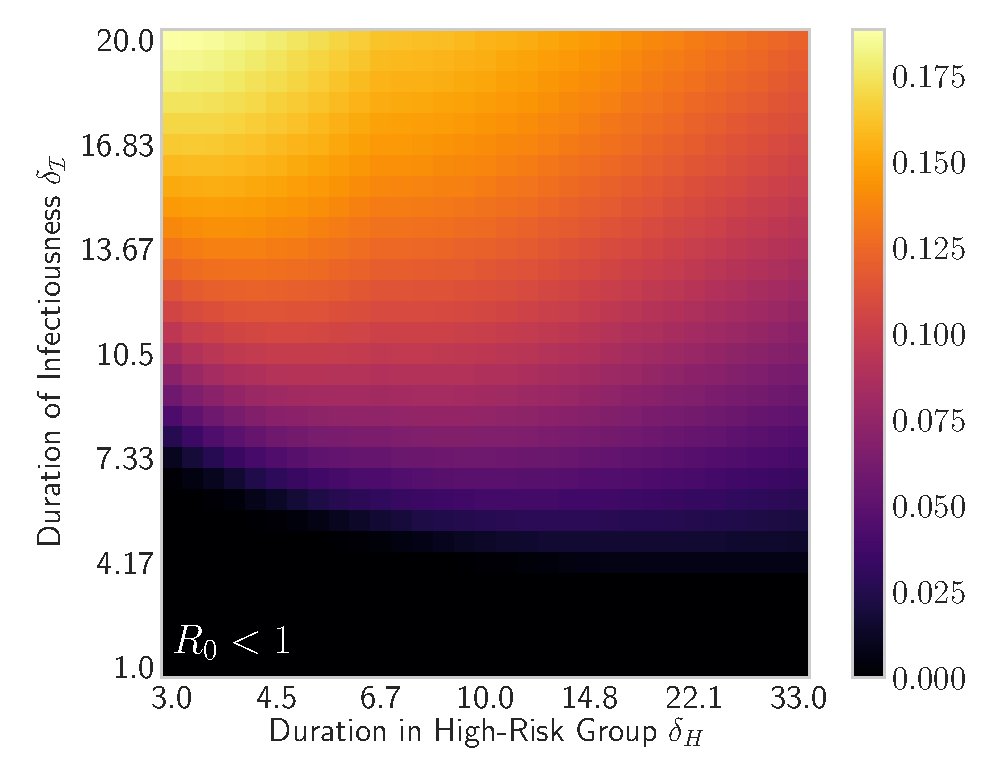
\includegraphics[width=\linewidth]{surface-prevalence-low}
    \caption{Low risk prevalence}
    \label{fig:surface-prevalence-low}
  \end{subfigure}
  \begin{subfigure}{0.31\linewidth}
    \centering
    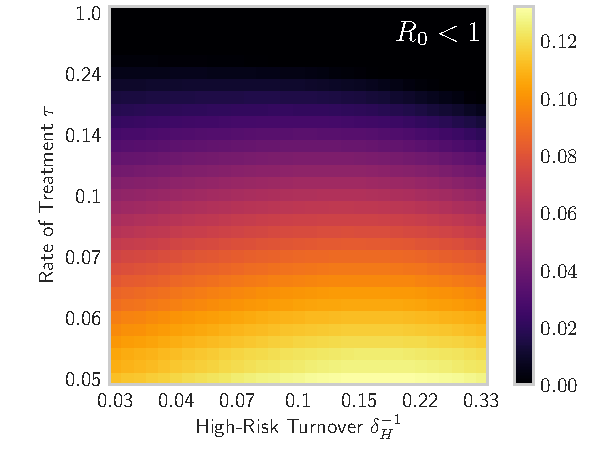
\includegraphics[width=\linewidth]{surface-prevalence-all}
    \caption{Overall prevalence}
    \label{fig:surface-prevalence-all}
  \end{subfigure}\\[1em]
  \begin{subfigure}{0.31\linewidth}
    \centering
    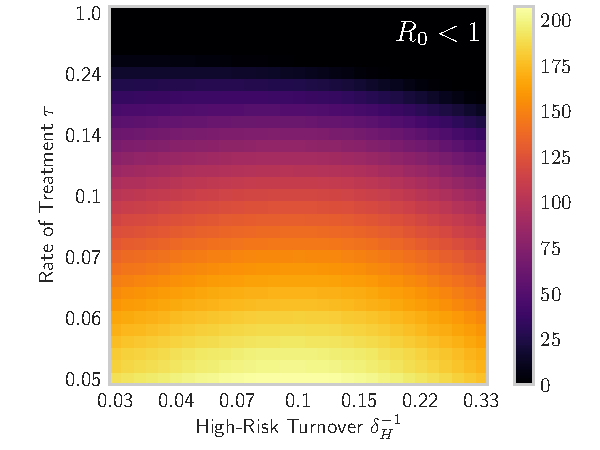
\includegraphics[width=\linewidth]{surface-incidence-high}
    \caption{High risk incidence}
    \label{fig:surface-incidence-high}
  \end{subfigure}
  \begin{subfigure}{0.31\linewidth}
    \centering
    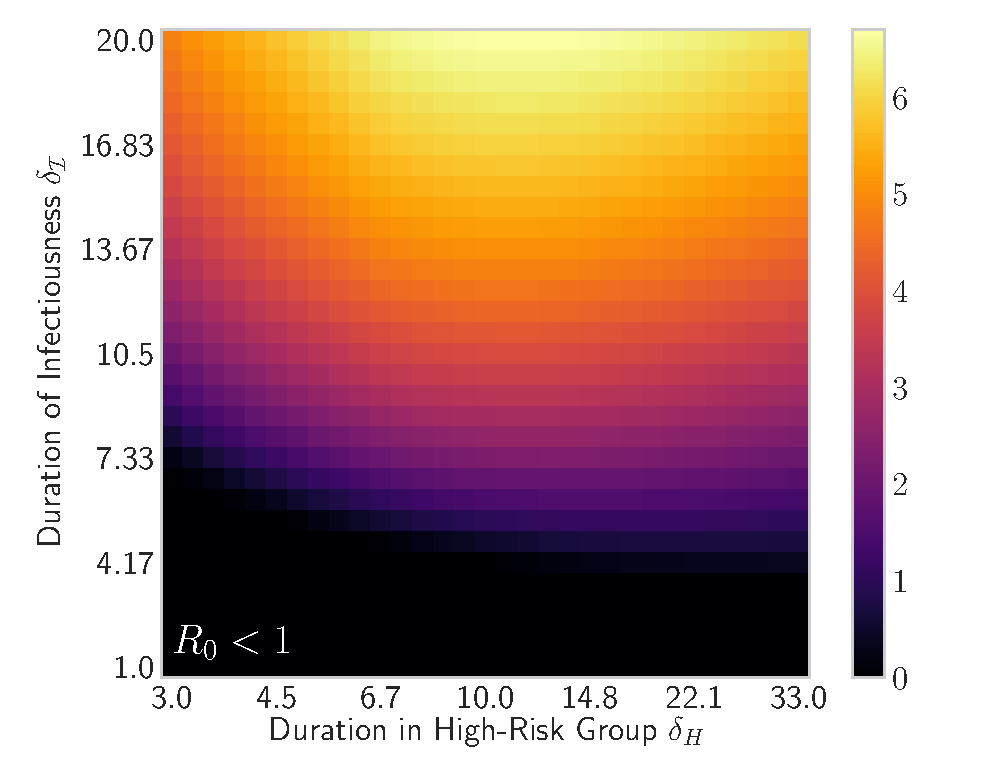
\includegraphics[width=\linewidth]{surface-incidence-low}
    \caption{Low risk incidence}
    \label{fig:surface-incidence-low}
  \end{subfigure}
  \begin{subfigure}{0.31\linewidth}
    \centering
    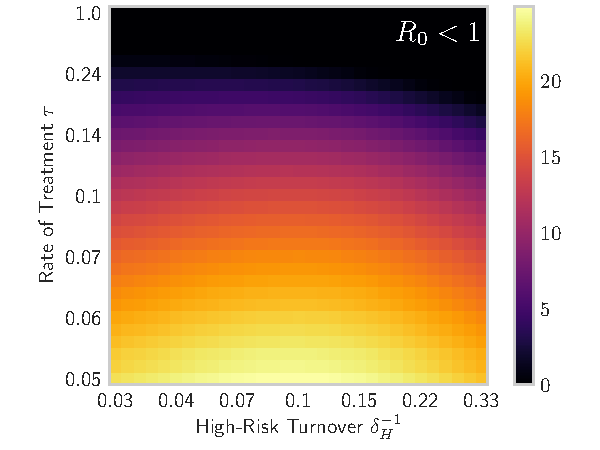
\includegraphics[width=\linewidth]{surface-incidence-all}
    \caption{Overall incidence}
    \label{fig:surface-incidence-all}
  \end{subfigure}
  \caption{Steady-state prevalence and incidence
    for different rates of turnover
    (based on $\delta_H$; log scale; turnover increases right to left)
    and duration of infectiousness $\delta_I$
    (reflecting treatment/disease course; linear scale; treatment increases top to bottom).}
  \label{fig:surface}
\end{figure}
% ==================================================================================================
\subsection{Fitted Models with Turnover}\label{ss:res-turnover-fit}
Model variants V1 (turnover) and V2 (no turnover) were both calibrated to
25\% and 5\% prevalence in the high and low risk groups, respectively,
by fitting the contact rates $C_i$.
The ratio between fitted high and low contact rates was much higher with turnover
($C_H / C_L = 
\input{\datapath/fit/nu=0.05_G=3_Z=1-CH.txt} /
\input{\datapath/fit/nu=0.05_G=3_Z=1-CL.txt} =
\input{\datapath/fit/nu=0.05_G=3_Z=1-CR.txt}$)
than without
($C_H / C_L =
\input{\datapath/fit/nu=0.05_G=3_Z=0-CH.txt} /
\input{\datapath/fit/nu=0.05_G=3_Z=0-CL.txt} =
\input{\datapath/fit/nu=0.05_G=3_Z=0-CR.txt}$).
This implies that, if turnover dynamics present in reality are not captured in the model,
the relative risk experienced by the high risk group
may be underestimated by calibrated models.
This is because, in order to observe
the same prevalence ratios between the high and low risk groups
in a system which has turnover,
the difference in risks experienced by each group would have to be larger,
since turnover acts to homogenize
the average risk experienced by each individual throughout their life.
\par
These dynamics also have implications
when estimating the TPAF of particular risk groups.
For instance, before model calibration, a system without turnover
estimates the TPAF of the high risk group to be greater than a system with turnover
(Figure~\ref{fig:tpaf-fit-from}, solid lines).
In this case, we think that
the high prevalence among the high risk group in the absence of turnover
maximizes incident infections \textit{from} the group,
yielding a higher TPAF.
However, after calibration of group-specific contact rates $C_i$,
the trend reverses, and the system with turnover predicts
a higher TPAF for the high risk group
(Figure~\ref{fig:tpaf-fit-from}, solid lines).
We hypothesize that this reversal is mainly attributable to
the larger ratio of fitted contact rates under turnover,
which dramatically increases the proportion of contacts (and therefore infections)
which occur with the high risk group.
Therefore, if real-world turnover processes are omitted from a calibrated epidemic model,
then the relative importance of reaching the high risk group with interventions
may be underestimated.
\begin{figure}
  \centering
  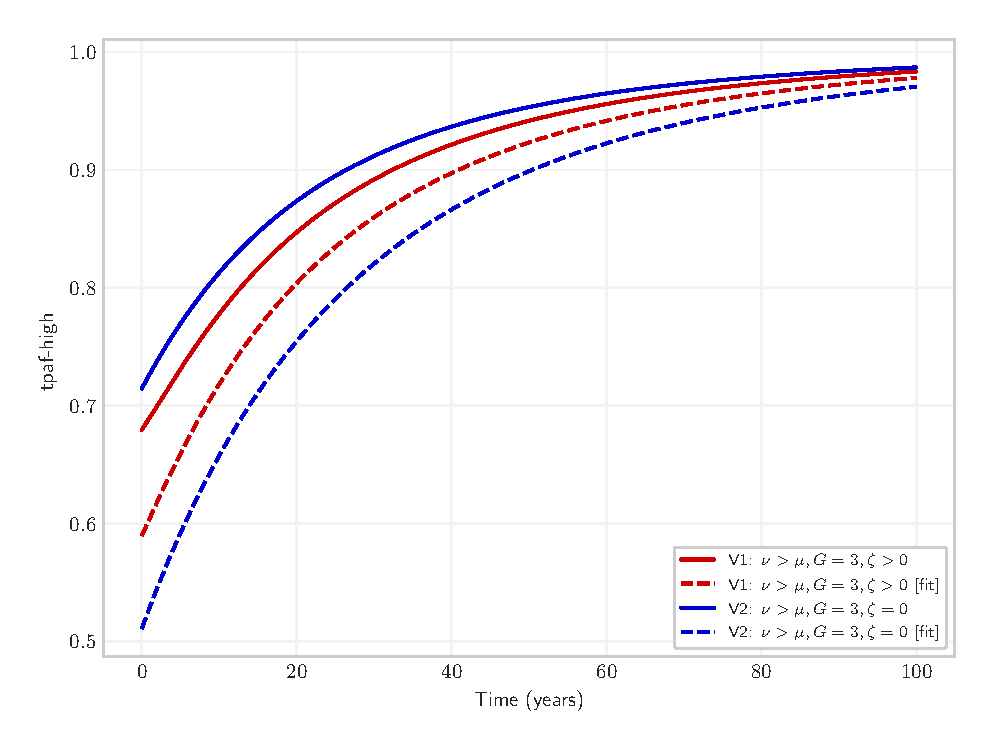
\includegraphics[width=0.6\linewidth]{compare-turnover-tpaf-fit-from}
  \caption{Transmission population attributable fraction (TPAF-from)
    of the high risk group with and without turnover,
    and with and without fitted $C_i$ to group-specific prevalence.}
  \label{fig:tpaf-fit-from}
\end{figure}